\documentclass[10pt,abstract=true,titlepage=false,toc=bib]{scrartcl}

\usepackage{fontspec}
\setmainfont{Libre Baskerville} % Libre Baskerville - Palatino Linotype - Constantia
\setsansfont{Helvetica} % Arial
\setmonofont{Consolas} % Hack

\usepackage[UKenglish]{babel}

\usepackage[margin=2.5cm]{geometry}

\usepackage{mathtools}
\usepackage{amssymb}
\usepackage{physics}
% \usepackage[version=4]{mhchem}
\usepackage[separate-uncertainty=true,per-mode=power]{siunitx} % ,per-mode=fraction 
% \usepackage{bm}


% \usepackage{url}
\usepackage{graphicx}
% \usepackage{float}
\usepackage{caption}
% \usepackage{subcaption}
\usepackage{booktabs}
\usepackage{csquotes}
% \usepackage{xcolor}
\usepackage[section]{placeins}



\usepackage{appendix}
% \usepackage[nottoc]{tocbibind}

% \usepackage[euler]{textgreek}


\usepackage{mgscience}

\usepackage[style=ieee]{biblatex} % ,sorting=none [style=alphabetic,defernumbers=true]
\bibliography{SCC}


\graphicspath{ {./images/} }


\usepackage{hyperref}
\hypersetup{
	colorlinks=true,
	linkcolor=blue,
	citecolor=cyan
}


\captionsetup[figure]{labelfont=bf,format=hang,labelsep=period,margin=1cm}
\captionsetup[table]{labelfont=bf,format=hang,labelsep=period,margin=1cm} % ,labelsep=newline


\renewcommand{\arraystretch}{1.2}

\parindent10mm


% \renewcommand{\thesection}{\thepart \arabic{section}.}
% \renewcommand{\thesubsection}{\thepart \arabic{section}.\arabic{subsection}.}
% \renewcommand{\thesubsubsection}{\thepart \arabic{section}.\arabic{subsection}.\arabic{subsubsection}.}



% \titlehead{\center test}

% \subject{Experiment 44}

\title{HiCRep: A Method of Comparing Hic Contact Matrices}


\author{Moritz Gmeiner}

\publishers{\vspace*{20pt} Supervisor: Peter Virnau}

\date{\today}

\begin{document}

\maketitle

\begin{abstract}

Using experiments and simulations, one can obtain contact matrices for the entire genome, detailing which sections of the genome are in contact with each other. HiCRep\cite{yang_hicrep_2017} introduces a measure called the stratum adjusted correlation coefficient (SCC) to compare the similarity between two such matrices. For this both contact matrices are first smoothed and the certain pearson correlation coefficients are calculated and weigthed average is performed.

\end{abstract}

\section{Method} % (fold)
\label{sec:method}

\subsection{Smoothing} % (fold)
\label{subsec:smoothing}

Both contact maps are first smoothed using a uniform filter of width \(2h+1\) for a chosen smoothing parameter \(h>0\). This helps dealing with a lack of coverage, that is the fact that not all actual contacts are contained in the contact matrices, something that is quite normal for Hi-C. Mathematically this filter is defined as

\[
	X_{ij} = \frac{ \sum_{k=i-h}^{i+h} \sum_{l=j-h}^{j+h} C_{kl} }{ 2h+1 }
\]

where \(C\) is the \(n \times n\) contact matrix and \(X\) is the \(n \times n\) smoothed matrix. \(C_{ij}\) is to be 0 for \(i\) or \(j\) not in \(1 \dots n\).

The uniform filter might seem like an unusual choice compared to other more sophisticated filters, but has the great advantage of having the representation \( X = L \cdot C \cdot R \), where \(C\) is the contact matrix to be smoothed, \(X\) is the smoothed matrix, and \(L\) and \(R\) are upper and lower trigangular matrices respectively. This comes in handy especially when using sparse representations of \(C\) and \(X\), as is very much recommended since contact matrices can generally be quite large and are largely empty.

\(h\) is a parameter for the SCC algorithm and thus has to be chosen appropriately. The HiCRep package includes a function called \verb|htrain| in the original R package (\verb|h_train| in the HiCRep.py python package) that tried to estimate an appropriate h-value heuristically. For our resolution of \(\SI{100}{kbp}\) an example value of \( h = 3 \) is given in the original HiCRep paper, which should be kept in mind as a refence later when trying to choose an h-value for our own data.

% subsection smoothing (end)

\subsection{SCC} % (fold)
\label{subsec:scc}

The stratum adjusted correlation coefficient aims to be a measure of correlation between two random variables \(X\) and \(Y\), stratified by a third variable into \(K\) strata \(X_1, \dots, X_K\) and \(Y_1, \dots, Y_K\) respectively. In each stratum we have the stratified random variables \((X_k, Y_k)\) with \(N_k\) observations \( (x_{k,1}, y_{k,1}), \dots, (x_{k,N_k}, y_{k,N_k}) \) each. The pearson correlation coefficient between \(X\) and \(Y\) for the k-th stratum is given by

\[
	\rho_k = \frac{ \mathrm{Cov}(X,Y) }{ \sqrt{ \mathrm{Var}(X) \mathrm{Var}(Y)} } = \frac{ \sum_{i=1}^{N_k} (x_{k,i} - \overbar{x}_k) (y_{k,i} - \overbar{y}_k) }{ \sqrt{ \sum_{i=1}^{N_k} x_{k,i} - \overbar{x}_k } \sqrt{ \sum_{i=1}^{N_k} y_{k,i} - \overbar{y}_k } }
\]

The SCC is the weighted average of the pearson correlation coefficients

\[
	\rho_s = \sum_{k=1}^{K} w_k \rho_k
\]

where the weights \(w_k\) are given as

\[
	w_k = \sqrt{ \mathrm{Var}\left( \frac{ \mathrm{Rank}(X_k) }{ N_k } \right) \mathrm{Var}\left( \frac{ \mathrm{Rank}(Y_k) }{ N_k } \right) }
\]

with \( \mathrm{Rank}(X_k) \) and \( \mathrm{Rank}(Y_k) \) being the ranked variables\footnote{\url{https://en.wikipedia.org/wiki/Ranking\#Ranking_in_statistics}}. For a thorough deviation of the SCC see \cite{yang_hicrep_2017}, Section \enquote{Derivation of stratum-adjusted correlation coefficient (SCC)}.

% subsection scc (end)

\subsection{Using SCC for comparison of Hi-C contact matrices} % (fold)
\label{subsec:scc_for_comparison_of_hi_c_contact_matrices}

To compare two Hi-C contact matrices we want to calculate SCC values for each chromosome. That is, for each chromosome we select the contact sub-matrix \(C\) that describes the contacts of that chromosome with itself. The observations of \(X\) and \(Y\) are the entries of these two sub-matrices, and the stratification is by genomic distances, that is \(\abs{j-i}\) for each contact \(c_{ij}\). In particular, the k-th stratum corresponds to the k-th diagonal in the contact sub-matrices. The original paper recommends limiting the maximum interaction range to \(\SI{5}{Mbp}\), which corresponds to a \(K\) of \(50\) in our \(\SI{100}{kbp}\) resolution. That means our SCC is actually a weighted average of the individual pearson correlation coefficients of the \(50\) first diagonals of the chromosome contact sub-matrices.

From these chromosomal SCC values then a total genomic SCC value can be calculated by again taking a weighted average, this time of the chromosomal SCC values using the chromosome lengths as weights. This will yield a value between \(-1.0\) and \(1.0\), with a value approching \(1.0\) meaning a high correlation between the contact matrices and one approaching \(0.0\) meaning little correlation (while negative values would be possible in theory they would be rather unusual, as a negative correlation would signal that each contact matrix's contacts are preferentially where the other matrix's contacts are not).

% subsection scc_for_comparison_of_hi_c_contact_matrices (end)

% section method (end)

\section{Analysis} % (fold)
\label{sec:analysis}

\subsection{Choice of h-value} % (fold)
\label{sub:choice_of_h_value}

For the choice of the h-value the \verb|h_train| function can be used. This functions repeatedly samples \(10\%\) of the contacts in both matrices, calculates the SCC and averages over them. This average SCC value will typically improve with larger values of h, and the \verb|h_train| function recommends the last h-value where the improvement is larger than \(0.01\). To train the h-value, the Hi-C contact matrix and the simulated contact matrix both of cell 2 were selected, since cell 2 provided very sensible data and those two contact matrices should be highly correlated. The average SCC value for the different h-values up to an h-value of \(10\) can be seen in Figure \ref{img:h_train}. One thing that immediately stands our is that there is actually a big drop from \(h=0\) to \(h=1\) and then the average SCC starts first rise and then plateau with the improvement becoming quite small. The recommended h-value is \(7\) which will be chosen for all subsequent SCC calculations.

\begin{figure}[ht]
\centering
	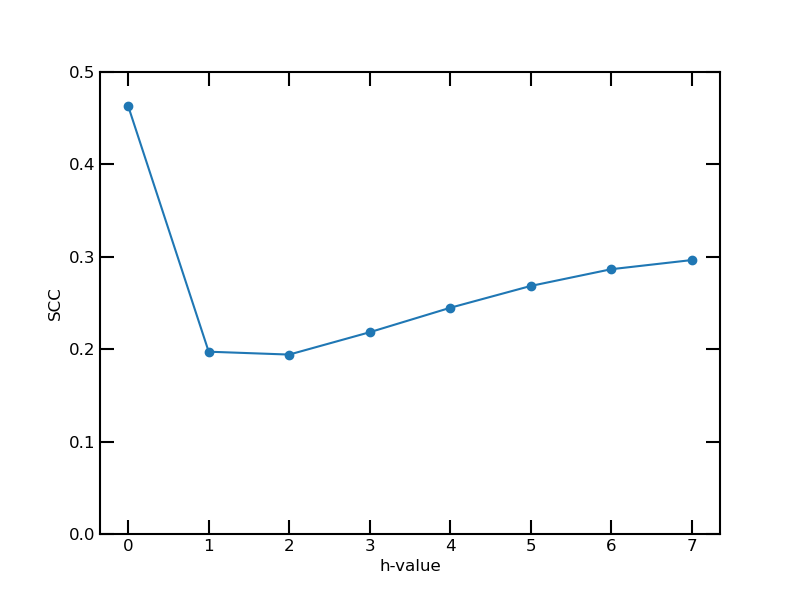
\includegraphics[width=14cm]{h_train.png}
	\caption{Average SCC over h-value. Reference data are the Hi-C contact matrix and the simulated contact matrix of cell 2, which are samples 100 times at 10\% for each h-value to then calculate an average SCC.}
	\label{img:h_train}
\end{figure}

% subsection choice_of_h_value (end)

\subsection{Hi-C vs simulated data} % (fold)
\label{sub:hi_c_vs_simulated_data}

In Figure \ref{img:hic-vs-sim-scc} the SCC between the original Hi-C contact matrices and the contact matrices of the simulation can be seen for each cell. For all cells the SCC is between \(0.68\) and \(0.80\). This is sensible since on one hand, the SCC is expected to be high, as the simulated data is based on the Hi-C data, on the other hand it is not surprising that the scores are not perfect since the Hi-C data doesn't cover all contacts in the real genome whereas the simulation data includes all contacts in the simulated genome.

\begin{figure}[ht]
\centering
	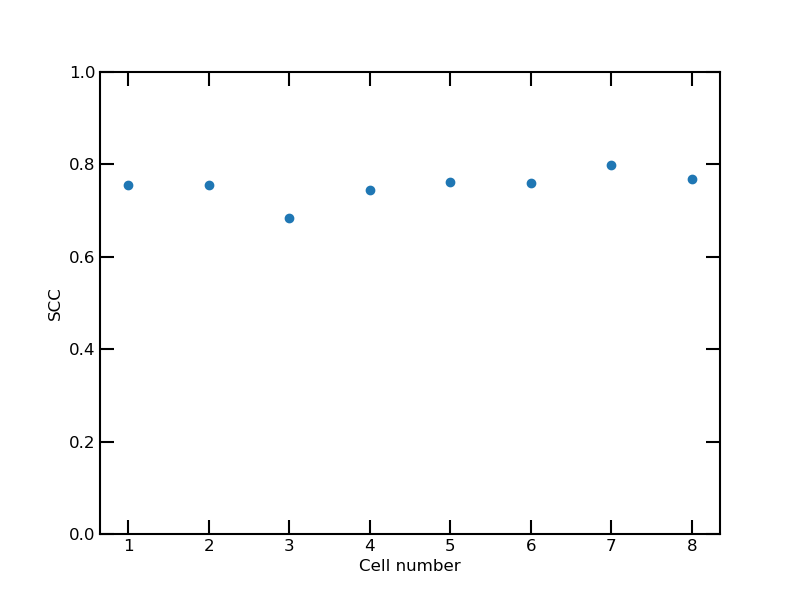
\includegraphics[width=14cm]{hic-vs-sim-scc.png}
	\caption{caption}
	\label{img:hic-vs-sim-scc}
\end{figure}

% subsection hi_c_vs_simulated_data (end)

\subsection{Comparison of different cells} % (fold)
\label{sub:comparison_of_different_cells}



% subsection comparison_of_different_cells (end)

% section analysis (end)

\newpage
\printbibliography

\end{document}